\section{Dynamic Scalable State Machine Replication}

In this section, we introduce Dynamic \ssmr{} (\dssmr), discuss performance optimizations, and argue about its correctness.

\subsection{General idea}
\label{sec:generalidea}

%S-SMR divides the state variables $v$ into $P$ partitions $\ppm_1, ..., \ppm_P$, where for each $\ppm_i$, $\ppm_i \subseteq \vvm$, and each variable $v$ in $\vvm$ has to be assigned to at least one partition and define $part(v)$ as the partitions that hold $v$. Each partition $\ppm_i$ is replicated by servers in group $s_i$. For brevity, the server $s$ belongs to $\ppm_i$ with the meaning that $s \in \ssm_i$, and say that client $c$ multicasts command $C$ to partition $\ppm_i$ means that $c$ multicasts $C$ to group $\ssm_i$.
%
%To execute command $C$, the client multicasts $C$ to all partitions that hold a variable read or updated by $C$.
%Consequently, the client must be able to determine the partitions accessed by $C$, denoted by $part(C)$. If the client cannot accurately estimate which partitions are accessed by $C$, it must determine a superset of these partitions, in the worst case assuming all partitions.
%In order for clients to provide a close approximation to the command's actually accessed partitions, there is an oracle that tells the client which partitions should receive each command.

Dynamic \ssmr\ (\dssmr) defines a dynamic mapping of variables to partitions.
Each variable $v$ is mapped to partition $part(v)$, meaning that $v \in part(v)$.
Such a mapping is managed by a partitioning oracle, which is implemented as a replicated service run by a group of processes.
The oracle service allows the mapping of variables to partitions to be retrieved or changed during execution.
In more detail, \dssmr\ distinguishes five types of commands:
$access(\omega)$ is an application command that accesses (reads or writes) variables in set $\omega \subseteq \vvm$ (as described in Section~\ref{sec:background}),
$consult(C)$ asks the oracle which variables are accessed by command $C$, and which partition contains each of them,
$create(v, \ppm)$ creates a new variable $v$ mapped to partition $\ppm$,
$move(v,\ppm)$ moves variable $v$ to partition $\ppm$,
and $delete(v)$ removes $v$ from the service state, resulting in $part(v) = \emptyset$.

% explain which partitions deliver each partitioning command:
% how are access, consult, create, move and delete implemented?

Once the oracle is in place, clients can consult it to know to which partitions each command should be multicast, based on which variables are accessed by the command.
If the reply received from the oracle tells the client that the command accesses a single partition, the client multicasts the command to that partition.
If the command accesses variables from multiple partitions, the client first multicasts one or more $move$ commands to the oracle and to the involved partitions, with the intent of having all variables in the same partition.
Then, the command itself is multicast to the one partition that now holds all variables accessed by the command.
If a subsequent command accesses the same variables, it will also access a single partition.
With this scheme, the access patterns of commands will shape the mapping of variables to partitions, reducing the number of multi-partition commands.

Consulting the oracle and issuing the application command are done with separate calls to atomic multicast in \dssmr{}.
It may happen that, between those operations, the partitioning changes.
We illustrate this in Figure~\ref{fig:move_case_1}.
Command $C_x$ reads the value of variale $x$.
Since partitioning is dynamic, the client issuing $C_x$ first consults the oracle and is told to multicast the command to $\ppm_1$.
However, before $C_x$ is multicast to $\ppm_1$, another client issues a $move$ command that relocates $x$ to $\ppm_2$.
When $C_x$ is delivered at the servers of $\ppm_1$, the command is not executed, since $x$ is not available at $\ppm_1$ anymore.
A similar situation may arise when a command accesses variables from multiple partitions, as it consists of multicasting at least three commands separately: $consult$, $move$ and $access$.
The parttioning can change between the execution of any two of those commands.

\begin{figure}[b!]
  \includegraphics[width=\linewidth]{figures/move_case_1}
  \caption{Consulting the oracle and issuing an application command consist of multiple calls to \amcast{}.}
  \label{fig:move_case_1}
\end{figure}

% TODO : mention retry x times

To solve this problem, \dssmr\ implements a versioning mechanism.
Each state variable $v$ has a version number $version(v)$ associated to it.
The reply from the oracle to each $consult$ request is called a $prophecy$. Each prophecy consists of a set of tuples $\langle v, \ppm, version(v) \rangle$, meaning that variable $v$ is mapped to partition $\ppm$ and its version number is $version(v)$.
If $v$ is not part of the service state (i.e., it was deleted or never created), the prophecy will contain $\langle v, \emptyset, 0 \rangle$.
Whenever a command that changes the partitioning is executed (i.e., $create$, $move$ or $delete$), a variable's version is changed in some way: a newly created variable has version $1$, moving a variable from one partition to another increments its version number, and deleting a variable reverts its version number to~$0$.

Consider the execution depicted in Figure~\ref{fig:read}~(a), where state variables $x$ is created on partition $\ppm_1$ in the middle of the execution of S-SMR. Command $C_1(x)$ and $C_3(x)$ reads the value of $x$, $C_2(x,\ppm_1)$ create $x$ on partition $\ppm_1$. Client a first multicasts query to the $Oracle$ for location of $x$, which is not available at that time, hence $Oracle$ return empty result, which tell client a to end the execution. Client b then wants to create variable $x$ on $\ppm_1$, before sending actual creating command, client b also multicasts query to $Oracle$ to get the involved partition (eg., $\ppm_1$), then multicasts $C_2(x,\ppm_1)$ to both $Oracle$ and $\ppm_1$. Oracle will update information of $x$, and $\ppm_1$ will execute create $x$ command. From then, for every read command to $x$ (eg., $C_3(x)$), $Oracle$ could answer with partition $\ppm_1$ which is the one holds $x$.

\begin{figure*}
\begin{minipage}[b]{1.0\linewidth} % A minipage that covers the whole width of the page
\centering
      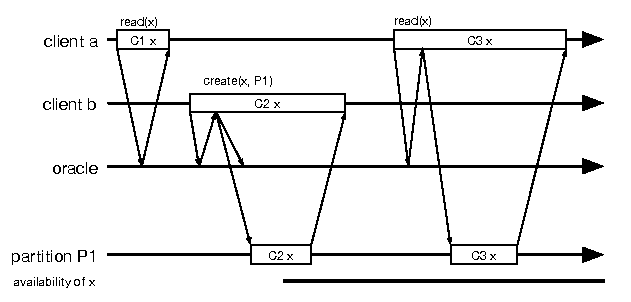
\includegraphics[width=0.6\linewidth]{figures/read_simple}
\end{minipage}
\centering
	\caption{Execution flow of DS-SMR with $create$ command}
\label{fig:read}
\end{figure*}

In the following figures~(\ref{fig:readoverlap}b, \ref{fig:readoverlap}c), where read command $C_1(x)$ comes in the middle of the execution of create command $C_2(x,\ppm_1)$, while the query of $C_1(x)$ comes after multicasts command of $C_2(x,\ppm_1)$. With the knowledge of $x$, Oracle response to the query with a positive answer, therefore there are possibilities that the read command either comes during (eg., fig.~\ref{fig:readoverlap}b) or before (eg., fig.~\ref{fig:readoverlap}c) the execution of actual write command. The SSMR model avoid the problem described in figure~\ref{fig:readoverlap}~(b) by ensuring that the execution of every command is atomic (eg., for every server $s$ in partition $\ppm$ that executes $C$, there is a server $r$ in every $\ppm' \in part(C)$ such that $delivery(C,r) < end(C,s)$. Intuitively, this condition guarantees that the execution of $C_1$ and $C_2$ at $\ppm$ overlap in time). Atomic multicast prevents the problem figure~\ref{fig:readoverlap}~(c) from happening as $deliver(C_2) \prec deliver(C_1)$, that leads to situation described in fig.~\ref{fig:readoverlap}b.

\begin{figure*}
\begin{minipage}[b]{1.0\linewidth} % A minipage that covers the whole width of the page
\centering
      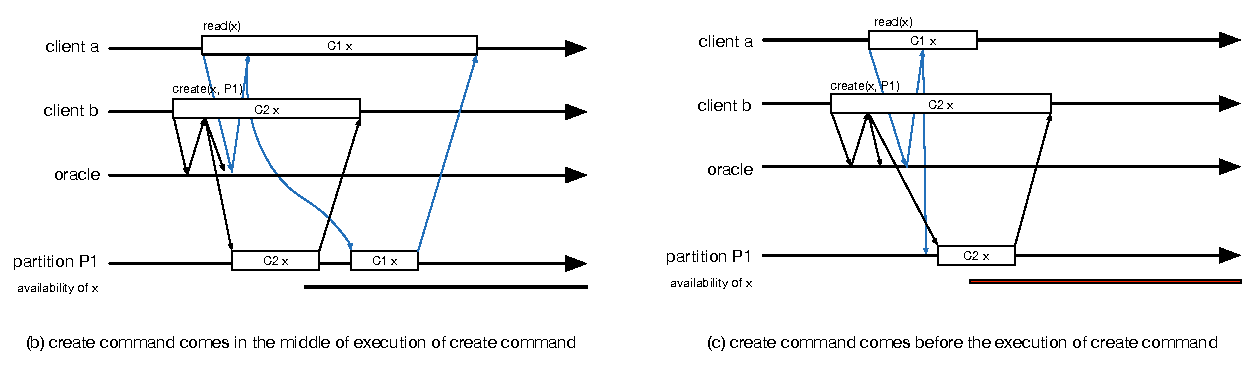
\includegraphics[width=1\linewidth]{figures/read_overlap}
\end{minipage}
\caption{Execution flow of D-SSMR with overlapping read-create commands}
\label{fig:readoverlap}
\end{figure*}


Next figure~(\ref{fig:updateoverlap} a, \ref{fig:updateoverlap} b) depicts the scenario of moving object location from a partition to another. Intuitively, the problem with the execution in fig.~\ref{fig:updateoverlap}a is that read command $C_3(x)$ executes “in between” the execution of $C_2(x,\ppm_2)$ at partitions Px and Py. Before sending $C_3$ to destination partition, client 1 send query to oracle for possible position of $x$, which is $P_1$ at that specific moment, but not correct at the execution time. In D-SSMR, we prevent that from happening by using oracle as the controller for accessing state variable on partitions, by using versioning mechanism on oracle for different type of commands. Whenever a client sends a command that update variable $C(x)$, oracle also increases the version of that variable $x$ in its knowledge. 
% Then after the associated process execute command $C$, it also tell Oracle to release the lock $L$, and inform the oracle about the update of $x$ (if there is any).

There are possibilities that a client could fail in the middle of the execution of the command chains, at the moment after requires the lock and before sending the actual $C$ command to partition $P$. In this case, TODO: which one release lock, either oracle or another client that require lock again. 

\begin{figure*}
\begin{minipage}[b]{1.0\linewidth} % A minipage that covers the whole width of the page
\centering
      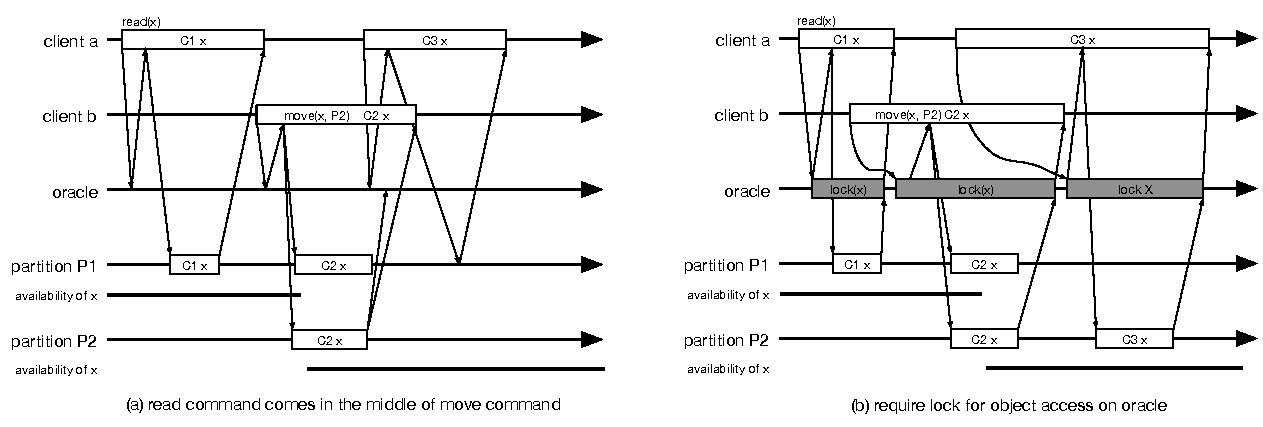
\includegraphics[width=1\linewidth]{figures/update_overlap}
\end{minipage}
\caption{Execution flow of DS-SMR with overlapping read-update commands}
\label{fig:updateoverlap}
\end{figure*}


\subsection{Detailed algorithm}
\label{sec:detailalg}

In Algorithm \ref{alg:dssmr}, we show the operation of DS-SMR. 
To submit a command $C$, the client first check its cache to get the lastest information $dests$ of the state objects in command. Then it can either uses that info if exists, or sends a query to the Oracle to get set $dests$~(line \ref{algline:query_oracle}, \ref{algline:oracle_response}), which is a superset of $part(C)$ used by the client as destination set for $C$~(line \ref{algline:cli_mcast}). 

Upon delivering $Q(C)$, oracle $O$ runs function $getPart(C)$ which returns a set $\vvm$ of involved state variables of command $C$. If there exists a variable $v_i \in \vvm$ in oracle memory, which indicates the variable $v_i$ exists on a partition $p_i \in \ppm$, oracle reply to client with $p_i$ value, or an empty result otherwise. In addition, upon delivering $C(v, \ppm)$, oracle update its memory with new location of $v$: $\vvm\_part\{v.id\} \leftarrow \ppm$

If the $dests$ from Oracle is empty, client stop the command there. (line \ref{algline:cli_terminate})

Upon delivering $C$, server $P$ execute $C$ and reply to the client. 
% Upon delivering $C$, server $s$ in partition \pp\ multicasts $signal(C)$ to $others$, which is the set containing all other partitions involved in $C$ (lines \ref{algline:others} and \ref{algline:mcastsignals}). 
% %The purpose of $signal(C)$ is to let servers in other partitions know that there is a server in \pp\ that started executing $C$. 
% It might happen that $s$ receives signals concerning $C$ from other partitions even before $s$ started executing $C$. For this reason, $s$ must buffer signals and check if there are signals buffered already when starting the execution of $C$. For the sake of simplicity, Algorithm \ref{alg:ssmr} simply initializes such buffers as $\emptyset$ for all possible commands. In practice, buffers for $C$ are created when the first message concerning $C$ is delivered.

% After multicasting signals, server $s$ proceeds to the execution of $C$, which is a sequence of operations that might read or write variables in \vv. The main concern is with operations that read variables, as they may determine the outcome of the command execution. All other operations can be executed locally at $s$. If the operation reads variable $v$ and $v$ belongs to \pp, $s$'s partition, then $s$ multicasts the value of $v$ to the other partitions that delivered $C$ (line \ref{algline:multicastv}). The command identifier $C.id$ is sent along with $v$ to make sure that the other partitions will use the appropriate value of $v$ during $C$'s execution. If $v$ belongs to some other partition $\ppm'$, $s$ waits until an up-to-date value of $v$ has been delivered (line \ref{algline:waitvariable}). Every other operation is executed with no interaction with other partitions (line \ref{algline:executeopck}).

% After executing all operations of $C$, $s$ waits until a signal from every other partition has been received (line \ref{algline:waitsignals}) and, only then, sends the reply back to the client (line \ref{algline:sendreply}). This ensures that $C$ will be execution atomic.



% Upon delivering $C$, server $s$ in partition \pp\ multicasts $signal(C)$ to $others$, which is the set containing all other partitions involved in $C$ (lines \ref{algline:others} and \ref{algline:mcastsignals}). 
% %The purpose of $signal(C)$ is to let servers in other partitions know that there is a server in \pp\ that started executing $C$. 
% It might happen that $s$ receives signals concerning $C$ from other partitions even before $s$ started executing $C$. For this reason, $s$ must buffer signals and check if there are signals buffered already when starting the execution of $C$. For the sake of simplicity, Algorithm \ref{alg:dssmr} simply initializes such buffers as $\emptyset$ for all possible commands. In practice, buffers for $C$ are created when the first message concerning $C$ is delivered.

\begin{algorithm}[h!]
\small

\begin{distribalgo}[1]

\vspace{1.25mm}

\INDENT{To issue a command $C$, the client proxy does:}

\vspace{1.0mm}

    \INDENT{\textbf{do}}
        \STATE \amcast$($oracle, $consult(C))$
        \STATE wait for $prophecy$
        \STATE $C.vars \leftarrow \{v: \exists P : \langle v, P \rangle \in prophecy \}$
        \STATE $C.dests \leftarrow \{P: \exists v : \langle v, P \rangle \in prophecy \}$
        \IF{$|C.dests| > 1$}
            \STATE $P_d \leftarrow$ one of the partitions in $C.dests$
            \FOR{every $v \in C.vars$}
                \STATE // \textit{move $v$ partition $P_d$}
                \STATE $P_o \leftarrow P : \langle v, P \rangle \in prophecy$
                \STATE $C_{move} \leftarrow move(v,P_d)$
                \STATE $C_{move}.dests \leftarrow \{$oracle$,P_o,P_d\}$
                \STATE \amcast$(C_{move}.dests$, $C_{move})$
            \ENDFOR
            \STATE $C.dests \leftarrow \{ P_s \}$
        \ENDIF
        \IF{$C$ is $create$ or $delete$}
            \STATE $C.dests \leftarrow dests \cup \{oracle\}$
        \ENDIF
        \STATE \amcast$(C.dests$, $C)$
        \STATE wait for reply
    \ENDINDENT
    \STATE{\textbf{while} reply = $retry$ // \textit{after $n$ retries, fall back to \ssmr}}
\ENDINDENT

\vspace{1.25mm}

\INDENT{To execute a command $C$, the server proxy in partition $P$ does:}

\vspace{1.0mm}

    \INDENT{\textbf{when} \amdel$(C)$, where $C$ is an $access$ command}
        \IF{$\exists v \in C.vars : v \not\in P$}
            \STATE reply with $retry$
        \ELSE
            \STATE have the command executed by the application server
            \STATE send the reply to the client
        \ENDIF
    \ENDINDENT

\vspace{1.0mm}
    \INDENT{\textbf{when} \amdel$(C)$, where $C$ is a $move$ command}
        \IF{$P_d = P$}
            \IF{$v \in P$}
                \STATE \rmcast$(P_d$,$\langle v, C \rangle)$
            \ELSE
                \STATE \rmcast$(P_d$,$\langle null, C \rangle)$
            \ENDIF
        \ENDIF
                \STATE wait until $\exists val : \langle val, C \rangle \in rcvd\_vars$
                \IF{$val \neq null$}
                    \STATE $P \leftarrow P \cup \{v\}$
                \ENDIF
    \ENDINDENT
\ENDINDENT

\caption{Dynamic \ssmr\ (\dssmr)}
\label{alg:dssmr}
\end{distribalgo}
\end{algorithm}

\subsection{Performance optimizations}
\label{sec:optm}

Algorithm 1 can be optimized in many ways. In this section, we briefly mention some of these optimizations and then detail caching.

Client can have a cache copy of the variable location on local. Thus when client issues command $C$, it does not need to query Oracle, instead it send a message direct to the associated partition based on its knowledge from cache. There are possibilities that client cache is invalid because of move command other client issued, thus the partition just need to return a response indicates invalid location. Then the client can retry the command by starting query from Oracle this time to get the updated location of state variable. 

\begin{figure*}
\begin{minipage}[b]{1\linewidth} % A minipage that covers the whole width of the page
\centering
      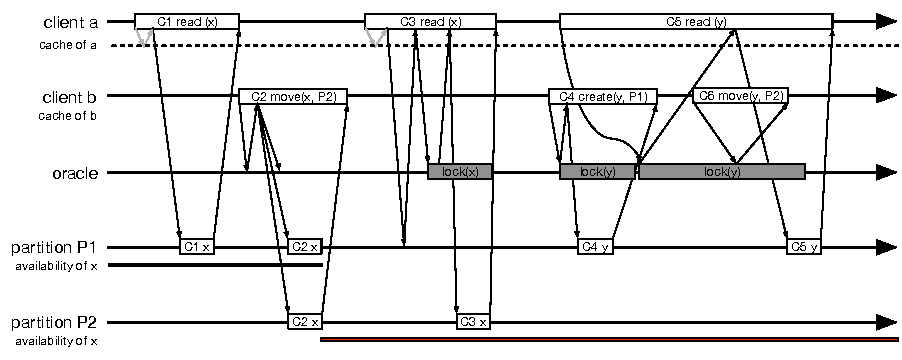
\includegraphics[width=0.85\linewidth]{figures/cache}
\end{minipage}
\caption{Execution flow of DS-SMR with oracle caching on client}
\label{fig:cache}
\end{figure*}

\subsection{Correctness}
\label{sec:correctness}
TODO: add content